\documentclass{article} % For LaTeX2e
\usepackage{nips15submit_e,times}
\usepackage{hyperref}
\usepackage{url}


\usepackage{amsmath,amsfonts,amsthm, amssymb} % Math packages
\usepackage{stmaryrd}
\usepackage[shortlabels]{enumitem}
\usepackage[pdftex]{graphicx}
\usepackage{booktabs}
\usepackage{placeins}
\usepackage{algpseudocode}
%\usepackage[margin=1in]{geometry}
\usepackage{listings}
\usepackage{mdframed}
\usepackage{tcolorbox}
\usepackage{float}
\usepackage{subcaption}
%\documentstyle[nips14submit_09,times,art10]{article} % For LaTeX 2.09


\title{RGB-D Object Recognition using Deep Learning}


\author{
Dario Aranguiz \\
University of Illinois at Urbana-Champaign \\
\texttt{arangui2@illinois.edu} \\
\And
Cu-Khoi-Nguyen Mac \\
University of Illinois at Urbana-Champaign \\
\texttt{knmac@illinois.edu} \\
}

% The \author macro works with any number of authors. There are two commands
% used to separate the names and addresses of multiple authors: \And and \AND.
%
% Using \And between authors leaves it to \LaTeX{} to determine where to break
% the lines. Using \AND forces a linebreak at that point. So, if \LaTeX{}
% puts 3 of 4 authors names on the first line, and the last on the second
% line, try using \AND instead of \And before the third author name.

\newcommand{\fix}{\marginpar{FIX}}
\newcommand{\new}{\marginpar{NEW}}

\nipsfinalcopy % Uncomment for camera-ready version

\begin{document}


\maketitle

\begin{abstract}
%!TEX root = ../final_report.tex

We implement a novel machine learning architecture to perform object recognition using color and low-resolution depth imaging. Our network utilizes pretrained networks for color and depth separately by transforming the depth frame into a color image, then fuses the classification results of the two networks using an additional fully connected layer. We achieve classification results of nearly 70\% and 80\% for the color and depth networks respectively, with less satisfactory results for the full fusion network discussed in the paper.

\end{abstract}

\section{Introduction}
%!TEX root = ../final_report.tex

\textit{Define and motivate the problem, discuss background material or related work, and briefly summarize your approach.}

Photography has remained generally unchanged since the first photograph was
taken in 1816 [todo ref]. The proceeding years since have seen a plethora of
technical advances bettering image quality, speed of image capture, as well as
other aspects, but imaging has remained a two-dimensional art. Developments in
recent years, however, have begun to fundamentally alter how we consider
imaging, with the release of the first Xbox Kinect in November 2010 [todo ref].
With this launch, consumers and researchers alike were able to view the world in
three dimensions, opening up a second modality to image processing.





\section{Details of approach}
%!TEX root = ../final_report.tex

\textit{Include any formulas, pseudocode, diagrams -- anything that is
necessary to clearly explain your system and what you have done. If possible,
illustrate the intermediate stages of your approach with result images.}

For our approach, we implemented a variation on the CVPR 2015 paper from Eitel
et al titled \textit{Multimodal Deep Learning for Robust RGB-D Object
Recognition} [todo ref]. The main contribution of this paper was to show how
pretrained networks such as AlexNet or VGGNet can be used to process single-
channel depth information, enabling networks to run on depth information
despite a lack of large-scale depth datasets such as ImageNet for color images
[todo ref]. In this section, we will discuss our network architecture, our
preprocessing phase, and our training methodology.


\subsection{Network Architecture}

The network structure proposed by Eitel et al [todo ref] is pictured in Figure
\ref{fig:network}. Its structure can be broken into three parts: a network for
color-based classification, a network for depth-based classification, and a
final fusion network combining the two single-modality streams into a final
classification result. Fusing two single-stream networks is beneficial for two
main reasons. Firstly, unlike large companies like Microsoft and Google who
have recently become involved in deep learning competitions, we do not have a
GPU farm at our disposal to train networks ad-infinitum. Additionally, the
first consumer depth camera was only released within the last 5 years [todo
ref]. Unlike ImageNet, we do not have millions of labeled depth captures to
use for network training. A smaller dataset could be used to train a depth
network from scratch, but using such a comparatively small dataset would
likely result in network overfitting and poor results on test data.

To this end, we use the pretrained network AlexNet for our single stream
network. AlexNet is a top-tier network without as many layers as a deep
residual learning network, making it a better choice for our limited compute
capacity and timeframe. Our implementation of AlexNet is shown in further
detail in Figure \ref{fig:single_stream_layout}. 

Finally, we strip the \texttt{fc8} classification layers from the our AlexNet streams and concatenate the two models, feeding the now 8092-node layer into \texttt{fc1-fus}, a 4096-node fully-connected layer. Lastly, this goes into a final classification layer with softmax activation.

\subsubsection{Convolutional Layer}

\subsubsection{ReLU}

\subsubsection{Batch Normalization}

\subsubsection{Max Pooling}





\begin{figure}
\begin{mdframed}
\begin{itemize}
    \item \texttt{conv-1}:
    \begin{itemize}
        \item $96 \times 11 \times 11$ Convolutional Filter
        \item ReLU Activation
        \item Batch Normalization
        \item $2 \times 2$ Max Pooling
    \end{itemize}
    \item \texttt{conv-2}:
    \begin{itemize}
        \item 2-width Zero Padding
        \item $256 \times 5 \times 5$ Convolutional Filter
        \item ReLU Activation
        \item Batch Normalization
        \item $2 \times 2$ Max Pooling
    \end{itemize}
    \item \texttt{conv-3}:
    \begin{itemize}
        \item 1-width Zero Padding
        \item $384 \times 3 \times 3$ Convolutional Filter
        \item ReLU Activation
    \end{itemize}
    \item \texttt{conv-4}:
    \begin{itemize}
        \item 1-width Zero Padding
        \item $384 \times 3 \times 3$ Convolutional Filter
        \item ReLU Activation
    \end{itemize}
    \item \texttt{conv-5}:
    \begin{itemize}
        \item 1-width Zero Padding
        \item $256 \times 3 \times 3$ Convolutional Filter
        \item ReLU Activation
        \item $2 \times 2$ Max Pooling
    \end{itemize}
    \item \texttt{fc6}:
    \begin{itemize}
        \item 4096-node Fully Connected Layer
        \item ReLU Activation
        \item 50\% Dropout
    \end{itemize}
    \item \texttt{fc7}:
    \begin{itemize}
        \item 4096-node Fully Connected Layer
        \item ReLU Activation
        \item 50\% Dropout
    \end{itemize}
    \item \texttt{fc8}:
    \begin{itemize}
        \item 51-node Fully Connected Layer
        \item Softmax Activation
    \end{itemize}
\end{itemize}
\end{mdframed}
\caption{Single-stream network layout for depth and color channels respectively. Dropout layers are removed during test time.}
\label{fig:single_stream_layout}
\end{figure}

\begin{figure}
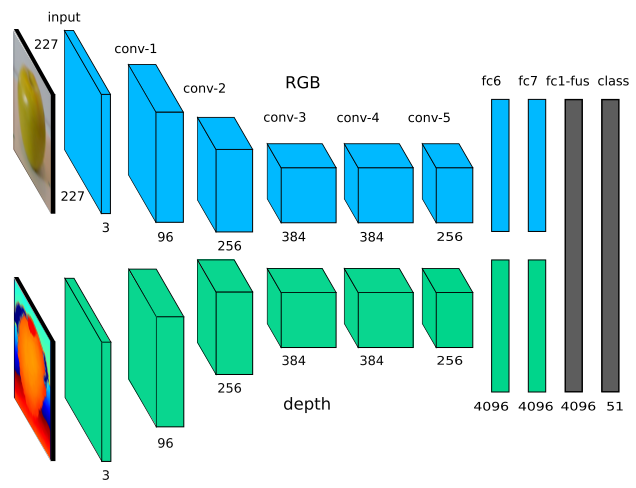
\includegraphics[width=\linewidth]{img/architecture.png} 
\caption{Network architecture using separate color and depth inputs. Inputs for color and depth are $227 \times 227 \times 3$, assuming depth colorization during preprocessing stage. Each modality has its own individual network, with the two resultant fusion layers providing final classification.}
\label{fig:network}
\end{figure}


\subsection{Preprocessing}

\subsection{Training}







\section{Results}
\textit{Clearly describe your experimental protocols. If you are using training and test data, report the numbers of training and test images. Be sure to include example output figures. Quantitative evaluation is always a big plus (if applicable). If you are working with videos, put example output on YouTube or some other external repository and include links in your report.}



\section{Discussion and conclusions}
%!TEX root = ../final_report.tex

\textit{Summarize the main insights drawn from your analysis and experiments. You can get a good project grade with mostly negative results, as long as you show evidence of extensive exploration, thoughtfully analyze the causes of your negative results, and discuss potential solutions.}

Our experimental results are not as accurate as they should be, but our single-stream depth network results are heartening. In particular, if we get $79.19\%$ accuracy from depth alone, our network should be able to at least show $79.19\%$ accuracy after the fusion layers. We were concerned that colorizing the depth map may add artificial information that would affect the results of the single-stream network, but there were no problems with the depth stream.

There is a suspicion that Keras is the current cause of our poor classification results. As mentioned earlier, a small refactoring which should not change the functionality of the architecture doubled our fusion classification rate. Our next steps, albeit after the course ends, will be to move our network to a different backend such as TensorFlow to see if that fixes any issues. We have considered other factors as well, namely:

\begin{itemize}
    \item \textbf{Implementation error}: It is tricky to show that we are not doing anything incorrect implementation-wise, but our single-stream network results validate the initial network setup and training phase. The second phase of training, freezing single-stream network weights, concatenating their outputs, and training the final fusion layers, are only a few lines of code. Unless we have missed something drastic, it is hard for something to go wrong in only a few lines.

    \item \textbf{Vanishing gradient}: A problem we had earlier during the semester was the issue of a vanishing gradient in the early layers. Adding batch normalization fixed the vanishing gradient and allowed us to train the full network.

    \item \textbf{Incorrect data coming from single-stream networks}: There may be a problem with the network concatenation such that the individual networks are not outputting correct data, but that issue was sorted when we switched from a Keras Sequential model to a Graph model.

\end{itemize}






\section{Individual contributions}
%!TEX root = ../final_report.tex

\textit{Required if there is more than one group member.}



\bibliographystyle{ieeetr}
\bibliography{mybib}


\end{document}
